\documentclass[a4paper,12pt]{article}

\topmargin -0.80cm \headheight 0.40cm \textwidth 15truecm
\textheight 24.4truecm

\usepackage[ansinew]{inputenc}
\usepackage{setspace}
\usepackage{lineno}
\usepackage{graphicx}
\usepackage{cite}
\usepackage{lscape}
\usepackage{amsfonts}

\begin{document}

\singlespacing

\newcommand{\cao}{\c{c}\~ao }
\newcommand{\coes}{\c{c}\~oes }
\newcommand{\caO}{\c{c}\~ao}
\newcommand{\coeS}{\c{c}\~oes}
\newcommand{\CAO}{\c{C}\~AO}
\newcommand{\COES}{\c{C}\~OES}
\newcommand{\cc }{\c{c}}
\newcommand{\CC }{\c{C}}
\newcommand{\y }{\'{\i}}
\def\gsim{\raise0.3ex\hbox{$\;>$\kern-0.75em\raise-1.1ex\hbox{$\sim\;$}}}

\def\binom#1#2{{#1\choose#2}}

%\begin{center}
%{\Large {\bf Letter to the Editor}}
%\end{center}
%\vskip 0.7cm

\vskip 1cm
\begin{center}
{\Large {\bf

Analysis of graphs generated by the number of divisors function
}}

\vskip 0.7cm

{\large {\rm B.L. Mayer$^{\rm{(a,1)}}$ and L.H.A.
Monteiro$^{\rm{(a,b,2)}}$}}


\vskip 0.5cm {\small

(a) Universidade Presbiteriana Mackenzie,

\vskip 0.05cm PPGEEC, S\~ao Paulo, SP, Brazil

\vskip 0.5cm (b)  Universidade de S\~ao Paulo,

\vskip 0.05cm Escola Polit\'ecnica, S\~ao Paulo, SP, Brazil


\vskip 0.5cm

\vskip 0.5cm (1) bleemayer@gmail.com

\vskip 0.1cm (2) luizm@mackenzie.br, luizm@usp.br }

\end{center}

\vskip 2cm

\begin{center}
{\it Corresponding author:}

\vskip 0.05cm Luiz Henrique Alves Monteiro

\vskip 0.05cm Universidade Presbiteriana Mackenzie

\vskip 0.05cm Escola de Engenharia

\vskip 0.05cm Rua da Consola\caO, n.896

\vskip 0.05cm 01302-907, S\~ao Paulo, SP, Brazil

\vskip 0.05cm E-mail addresses: luizm@mackenzie.br, luizm@usp.br

\vskip 0.05cm Telephone number: (55)(11)2114-8711

\vskip 0.05cm Fax number: (55)(11)2114-8600

\vskip 1cm ORCID ID: 0000-0002-2309-1254
\end{center}


\newpage

\section{Introduction}

This paper presents studies on two series generated using the divisor
function.

The first is generated by the points $(x,|\{d : d|x\}|)$ for $n\in N$
that is: each number to its quantity of divisors. That is:
$$\{(2,2), (3,2), (4,3), (5,2),\ldots, (10000,25)\}$$

The second applies the divisor function iteratively until the result reaches
2, that is, is a prime number, this series will be called as the orbit series
through this paper. For example, take the number 60:

\begin{itemize}
    \item 60 has 12 divisors, first time
    \item 12 has 6 divisors, second time
    \item 6 has 4 divisors, third time
    \item 4 has 3 divisors, fourth time
    \item and finally, 3 has 2 divisors, fifth time
\end{itemize}

Is this case we applied the function 5 times, hence the orbit of 60
has length 5, and the point is $(60, 5)$. Generating the following sequence:
$$\{(2,1), (3,1), (4,2), (5,1),\ldots, (10000,3)\}$$

The intention is to discover for each case how the natural visibility and
horizontal visibility measures relate. And in consequence, how the two
series are related.

Also, for the two cases the mean shortest path was calculated at each new
vertex.

\section{Methodology and numerical results}

This section describes the procedure to build and analyse each series.
The analysis consists of calculating the natural and horizontal visibilities
for the series, then fitting the model $Cx^{-\gamma}$ on the degree distribution
of the generated graph and analyse the coefficients.

In the studies the numbers started at 2 to avoid the only case of 1
divisor. On the second study specifically, the orbit of 2 was set to 1
instead of 0 to avoid this special case and, as consequence, dividing
the graph in two disconnected subgraphs.
All links are considered undirected.

The following table summarizes the parameter values of the two studies.

\begin{equation}
    \begin{array}{l|l|c|c}
       \textrm{series} & \textrm{visibility} & \gamma & C \\
        \hline
        \textrm{divisors} & \textrm{natural} & 1.21489 \pm 0.18265 & 0.559692 \pm 0.132711 \\
        \textrm{divisors} & \textrm{horizontal} & 0.637136 \pm 0.658635 & 0.190621 \pm 0.174726 \\
        \textrm{orbits} & \textrm{natural} & 0.556285 \pm 0.414888 & 0.149885 \pm 0.0999156 \\
        \textrm{orbits} & \textrm{horizontal} & 0.353234 \pm 1.56196 & 0.198959 \pm 0.379138 \\
    \end{array}
\end{equation}


In the following paragraphs all results for the two studies are displayed,
for each set we show first the graph, for illustration purposes, 
then the plot of the mean shortest path.


The figure (1) shows a graph that is generated using the divisors
series, by adding links $(x,y)\mapsto x\to y$

\begin{figure}[h!]
    \centering
    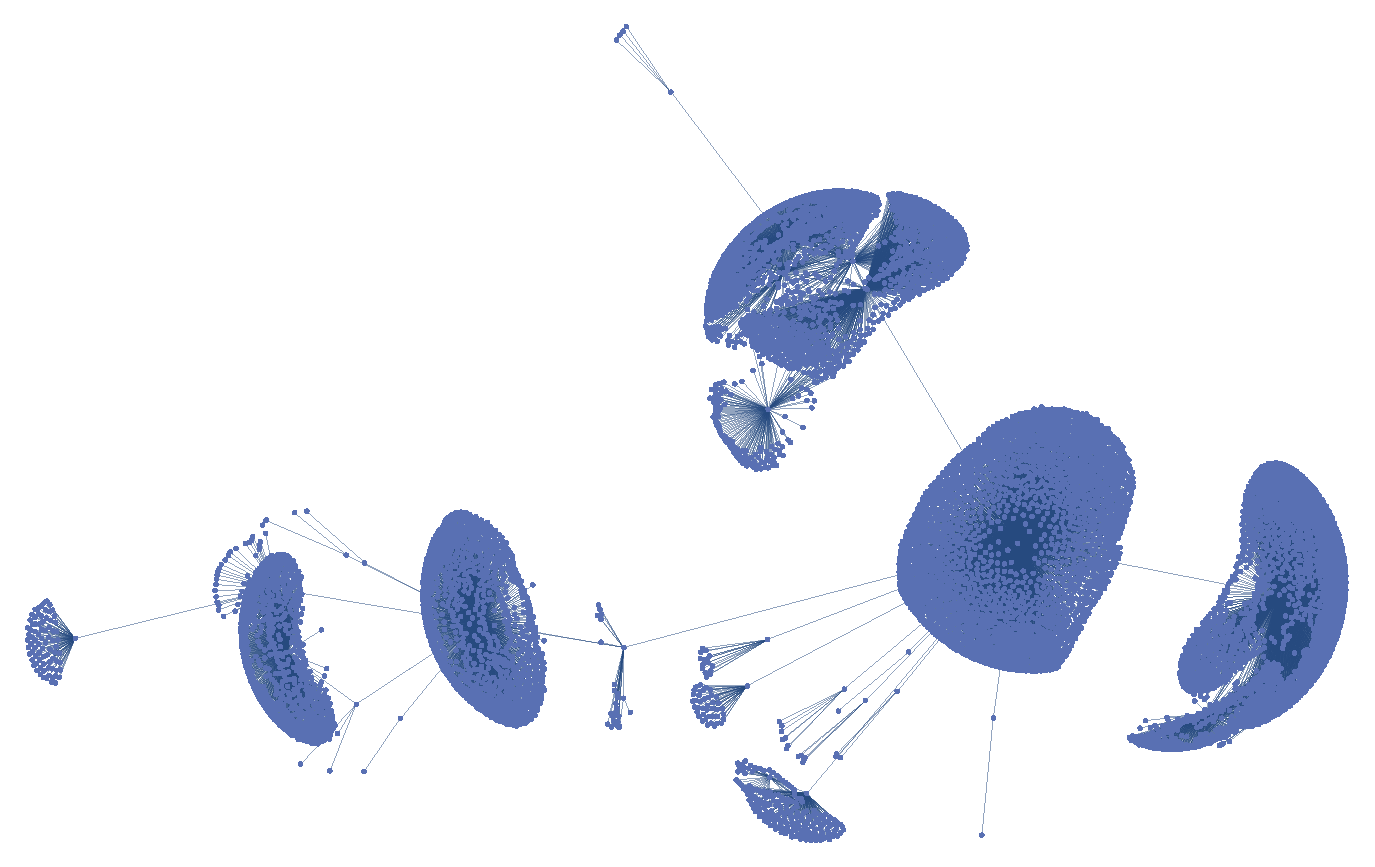
\includegraphics[width=0.75\textwidth]{divisors.pdf}
    \caption{Graph illustrating the divisors series}
    \label{graphs}
\end{figure}


The figure (2) shows the corresponding plot of mean shortest path
in relation to the number of nodes for the divisors series.

\begin{figure}[h!]
    \centering
    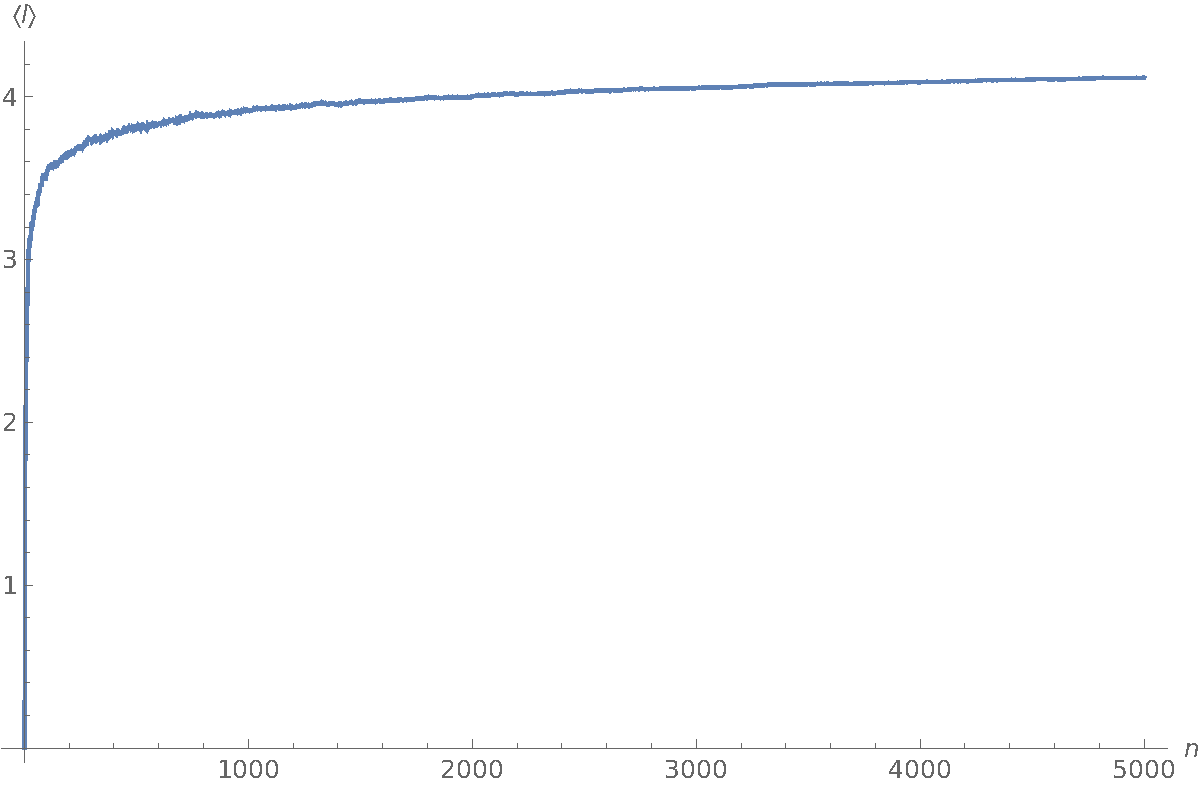
\includegraphics[width=0.75\textwidth]{growth-divisors.pdf}
    \caption{Graph of the mean shortest path for each new vertex up to 5000 nodes}
    \label{graphs}
\end{figure}


The figure (3) shows the graph generated by the orbits series.

\begin{figure}[h!]
    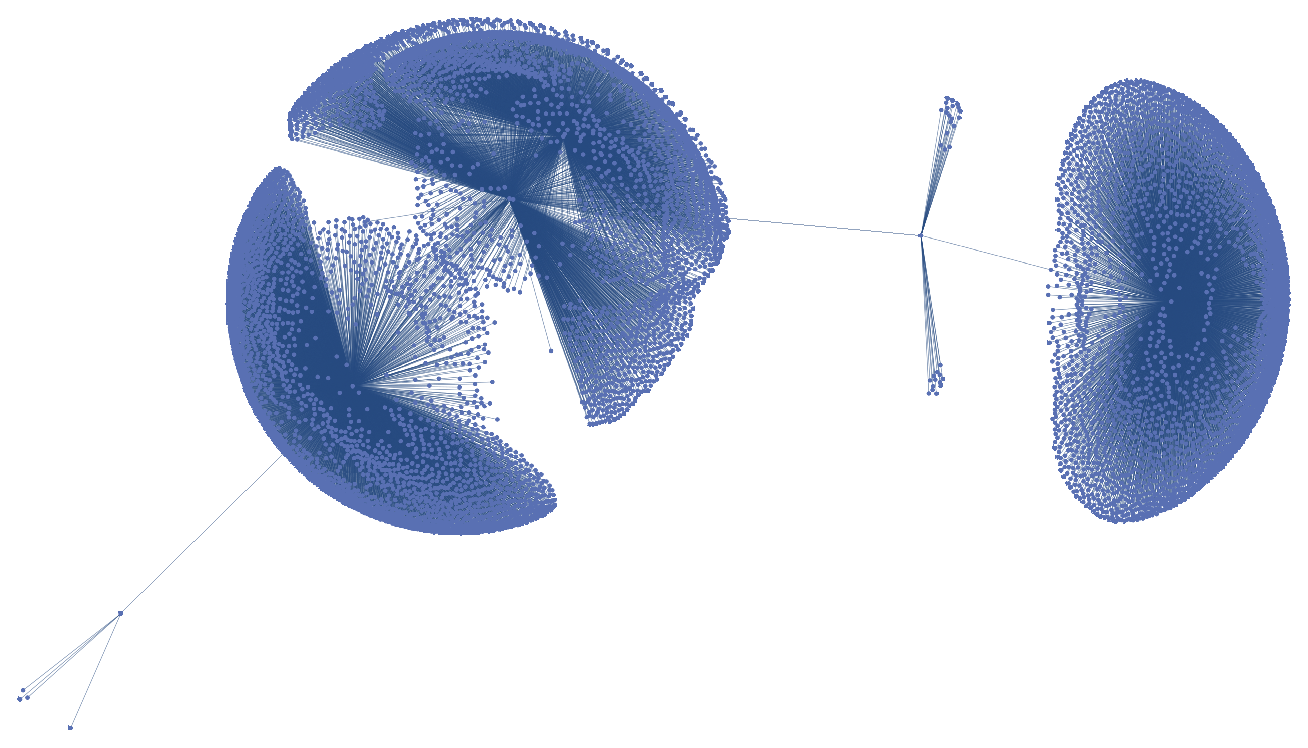
\includegraphics[width=0.75\textwidth]{orbits}
    \centering
    \caption{Graph illustrating the orbits series}
    \label{frame}
\end{figure}


And figure (4), the corresponding plot of mean shortest path.

\begin{figure}[h!]
    \centering
    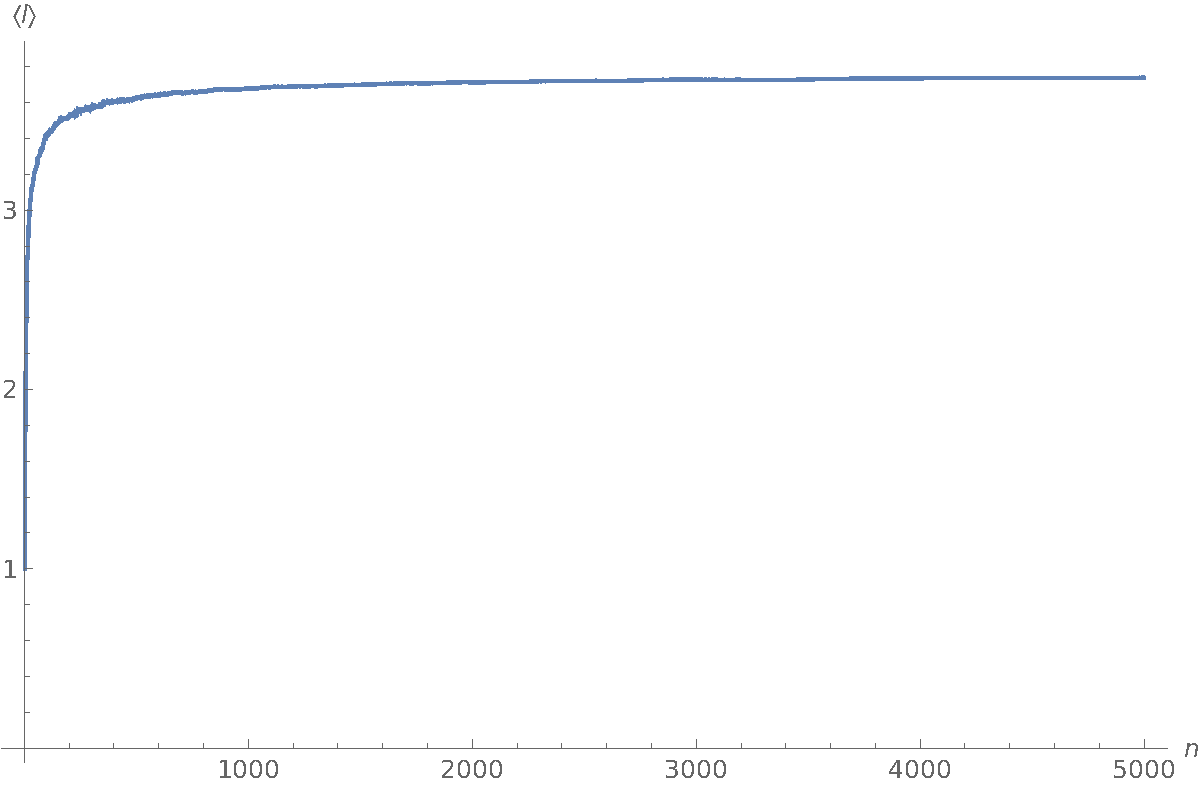
\includegraphics[width=0.75\textwidth]{growth-orbits.pdf}
    \caption{Graph of the mean shortest path for each new vertex up to 5000 nodes}
    \label{graphs}
\end{figure}


\section{Discussion and Conclusion}

By visual inspection the graphs are alike, they show a fractal structure and
the associated $\gamma$ coefficient for the orbits series is approximately
half of the divisors series, but has shown a big variance, which indicates
that the model may not be the best choice.

In the two studies the mean minimum path seemed to converge, the divisors
series converges to $4.11735$ and the orbits series to $3.73921$. Using more
nodes can increase the precision, in the divisor series the value seems to take
longer to converge.

In both cases the number of nodes can be increased to give more precise
results, also the orbit of the orbit can be studied.

A possible further study is to determine the likelihood of a node forming
a link with the new node during the construction of a graph. This can
lead to the values of convergence of the mean minimum path for both graphs.


\end{document}
